\chapter{Architettura hardware e software}

\section{Hardware}
\subsection{Premessa}
Per l'implementazione dell'architettura hardware è stata utilizzata della componentistica semplice ed economica. Principalmente l'hardware utilizzato è un \textit{Raspberry} ed un \textit{ricevitore GPS}, per ricevere le coordinate geografiche della barca durante la competizione.

\subsection{Raspberry}
A bordo della barca è stato installato un \textbf{Raspberry Pi 3 Model B}, un computer di dimensioni ridotte (\textit{single board computer}) che non necessita di eccessivi consumi di energia elettrica e dal costo contenuto. La particolarità di non avere della componentistica di alto livello permette di eseguire un qualsiasi sistema operativo basto su kernel Linux, fornendo un enorme vantaggio dal punto di vista del consumo energetico. Essendo la barca a vela il contesto in cui viene utilizzata questa \textit{single board}, non vi è la possibilità di fornire grandi quantità di energia per sostenere il carico energetico di hardware di alto livello. Pertanto la durata della batteria è un aspetto di fondamentale importanza.

\newpage
Il modello del Raspberry in questione ha le seguenti caratteristiche:
\begin{enumerate}
	\item CPU Quad Core 1.2GHz Broadcom BCM2837 a 64bit
	\item 1GB di RAM
	\item Modulo WLAN BCM43438 e \textit{Bluetooth Low Energy} (BLE) integrato
	\item 10/100 Fast Ethernet
	\item 2 porte USB 2.0
	\item Uscita video HDMI
	\item Lettore schede Micro SD integrato dove risiede il sistema operativo
	\item Porta di alimentazione Micro USB
\end{enumerate}

Il Raspberry deve ospitare un'applicazione server che fornirà dei servizi ai client, comunicare con i vari sensori installati nella barca a vela e mantenere attiva una rete WiFi a cui i vari client possono connettersi per accedere ai servizi del server. Quindi, il Raspberry ha anche il ruolo di \textit{access point wireless}.

\begin{figure}
	\begin{center}
		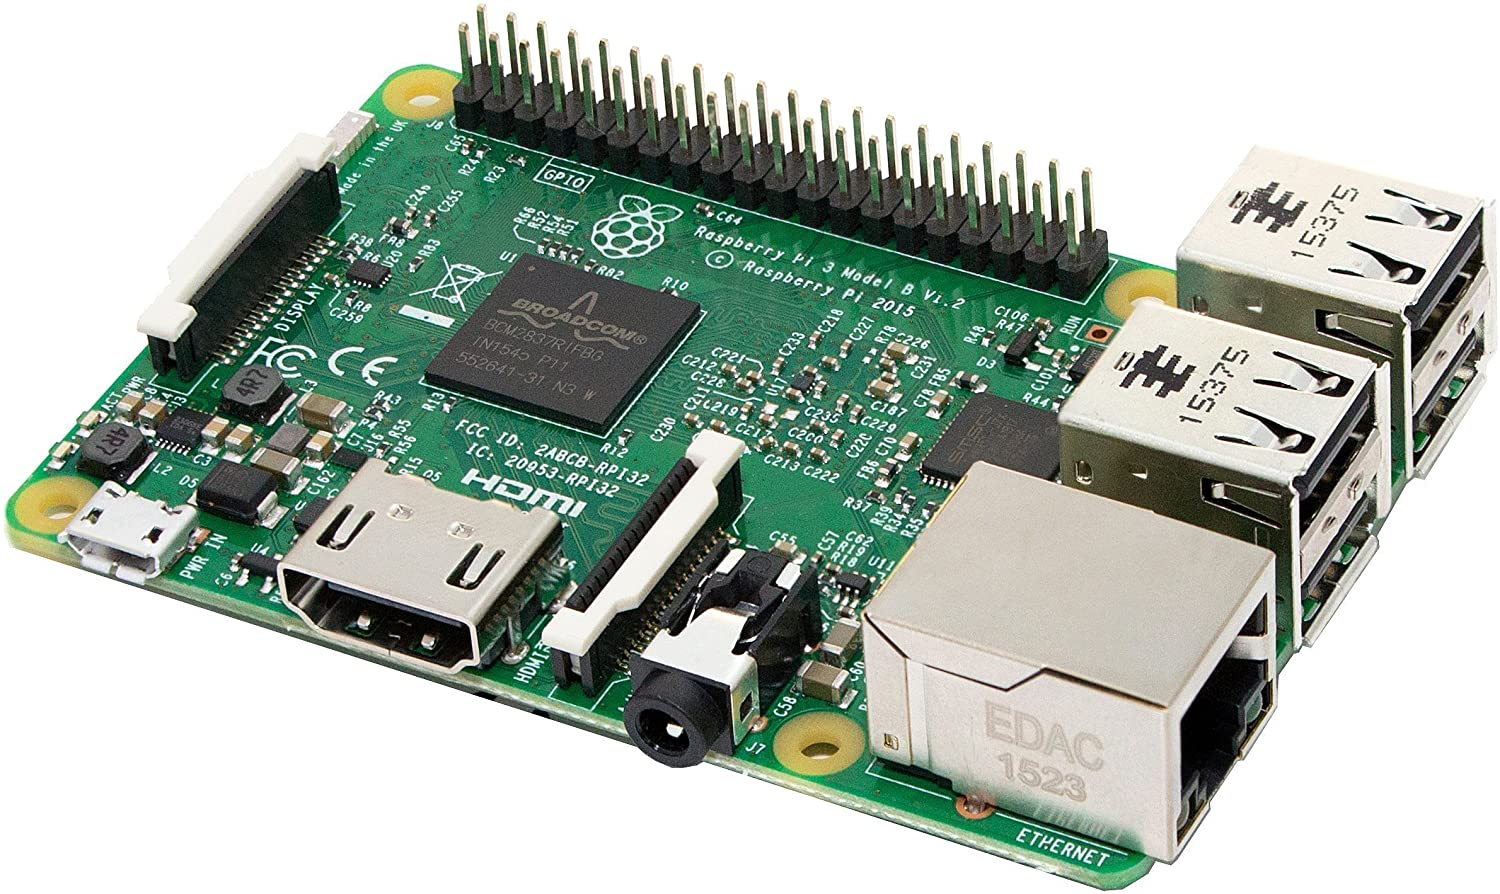
\includegraphics[scale=0.2]{raspberry}
		\caption[Raspberry Pi 3 Model B]{Raspberry Pi 3 Model B.}
		\label{figura:raspberry}
	\end{center}
\end{figure}

\newpage
\subsection{Ricevitore GPS}
Per tracciare la rotta da percorrere è necessario ottenere le coordinate geografiche, fornite tramite il \textit{servizio GPS} \cite{gps}. Pertanto viene utilizzato un ricevitore GPS a basso costo, collegabile via USB al Raspberry. L'utilizzo del GPS risulta essere lo strumento ideale in questo contesto, in quanto, trovandosi in un'ampia area, gli eventuali errori vengono mitigati e non compromettono la precisione della posizione determinata.
\begin{figure}
	\begin{center}
		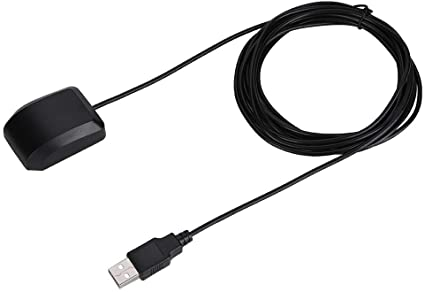
\includegraphics[scale=0.6]{gps_usb}
		\caption[Ricevitore GPS]{Ricevitore GPS collegabile via USB.}
		\label{figura:gps_usb}
	\end{center}
\end{figure}

\section{Software}
\subsection{Modello architetturale}
Per questo progetto si è deciso di utilizzare un'architettura \textbf{Client-Server}. È un modello architetturale per sistemi distribuiti dove le funzionalità che offre il server sono presenti sotto forma di servizi disponibili ai client. I client accedono al server per usufruire dei servizi offerti.

Il principale vantaggio che si può trarre da questa architettura è la possibilità di accedere al server da più postazioni. In questo progetto risulta molto utile accedere al server da postazioni differenti o supportare connessioni multiple (utilizzare l'applicazione da mobile e l'applicazione Web).
L'indipendenza tra server e client è un importante vantaggio in quanto è possibile apportare delle modifiche ad uno dei due \textit{attori} senza influire sull'altro o su altre parti del sistema. I client devono conoscere il nome del server disponibile (o i nomi dei server nel caso in cui ve ne siano più di uno) e i servizi che offre. Il server invece non necessita di conoscere i client che si connettono a lui ed è in grado di gestire un numero arbitrario di connessioni. I client usufruiscono dei servizi offerti dal server tramite un protocollo di \textit{richiesta-risposta}, dove un client invia una richiesta e rimane in attesa di una risposta da parte del server. In particolare, il protocollo implementato per questo progetto permette la comunicazione tra i due attori tramite l'utilizzo delle \textit{socket}, un'astrazione che fornisce una API per l'architettura TCP/IP.

Lo svantaggio maggiore di questa architettura è la suscettibilità ad attacchi \textit{Denial-of-Serevice} (\textit{DoS}), oltre ad essere soggetta ad eventuali guasti del server. Inoltre le prestazioni possono essere imprevedibili in quanto dipendono sia dal carico della rete, sia dal carico di lavoro che il server deve sostenere.

È necessario prestare attenzione alla separazione tra il concetto di \textit{server fisico} e l'\textit{applicazione server}: il server fisico è una macchina fisica dotata di componentistica in grado di poter supportare le funzionalità tipiche di un server (grandi quantità di risorse di calcolo e di memoria). L'applicazione server è un software che fornisce dei servizi per i client e che può essere installato indipendentemente che il dispositivo sia un server fisico o un normale personal computer. Un discorso analogo può essere fatto anche per i client.

\subsection{Funzionalità implementate dal server}
\subsubsection{Comunicazione con i sensori}
Una delle funzionalità principali che il server implementa è la comunicazione con i sensori installati sulla barca a vela. In particolare, il server raccoglie i dati in tempo reale, leggendoli in \textit{modalità seriale}. La comunicazione tra il server ed i sensori avviene tramite la centralina \textbf{NMEA 183 Interface Output}, sviluppata dall’azienda \textit{NKE Marine Electronics}. Questa centralina opera da intermediario tra i dati rilevati dai sensori ed il Raspberry. In particolare, la centralina converte i dati che provengono dai sensori in formato \textit{ASCII} e li trasmette tramite la porta seriale al server, utilizzando il formato \textbf{NMEA 0183}, un formato standard di comunicazione utilizzato per applicazioni nautiche e per dati GPS.

\newpage

\subsubsection{Manipolazione dei dati raccolti}
Una volta prelevati i dati dai sensori, questi vengono memorizzati in un \textit{buffer}, pronti per essere inviati ad un qualsiasi client che ne fa richiesta. I dati vengono parsati in JSON, un formato per lo scambio di informazioni molto usato per le comunicazioni di rete. Inoltre, i dati prelevati dai sensori vengono utilizzati per la generazione di file di \textit{log}, necessari per eseguire delle simulazioni a terra.

\subsection{Argos}
Sul Raspberry è stato installato il software \textbf{Argos}. Argos è un'applicazione lato server che offre dei servizi ai client che vi si connettono. È scritto in \textit{C} e permette di raccogliere i dati registrati dai sensori installati sulla barca. Questi dati vengono notificati dai sensori al server ad intervalli regolari, in modo da averli sempre aggiornati ai fini delle decisioni che devono essere prese durante la competizione. Per rendere disponibili questi dati ai client, Argos apre una socket nella rete locale e rimane in ascolto sulla porta \verb|4545|: appena un client si connette, il server restituisce il set di dati formattato in JSON e chiude la comunicazione, ritornando in ascolto sulla porta.

\subsubsection{Prima versione}
La prima versione dell'applicazione server rimaneva in ascolto su due porte: la porta \verb|4545| e la porta \verb|4546|. Tramite la porta \verb|4545|, venivano accettate le richieste dei client che volevano ottenere le informazioni riguardo ai sensori della barca in formato JSON. Tramite la porta \verb|4546|, invece, i client potevano inviare delle richieste in formato JSON, differenti rispetto alle prime. Queste richieste indicavano al server di svolgere determinate azioni. Quindi, le richieste venivano elaborate dal server e la risposta veniva fornita tramite la porta \verb|4545|.

\subsubsection{Seconda versione}
La seconda versione del server ha rimosso la funzionalità della porta \verb|4546|, ovvero, è stata tolta la possibilità di ricevere dei dati da parte dei client, di elaborarli e di restituire una risposta. Quindi, l'ultima versione permette soltanto di connettersi alla porta \verb|4545| per ottenere i dati provenienti dai sensori della barca, parsati e formattati dal server.

\begin{figure}
	\begin{center}
		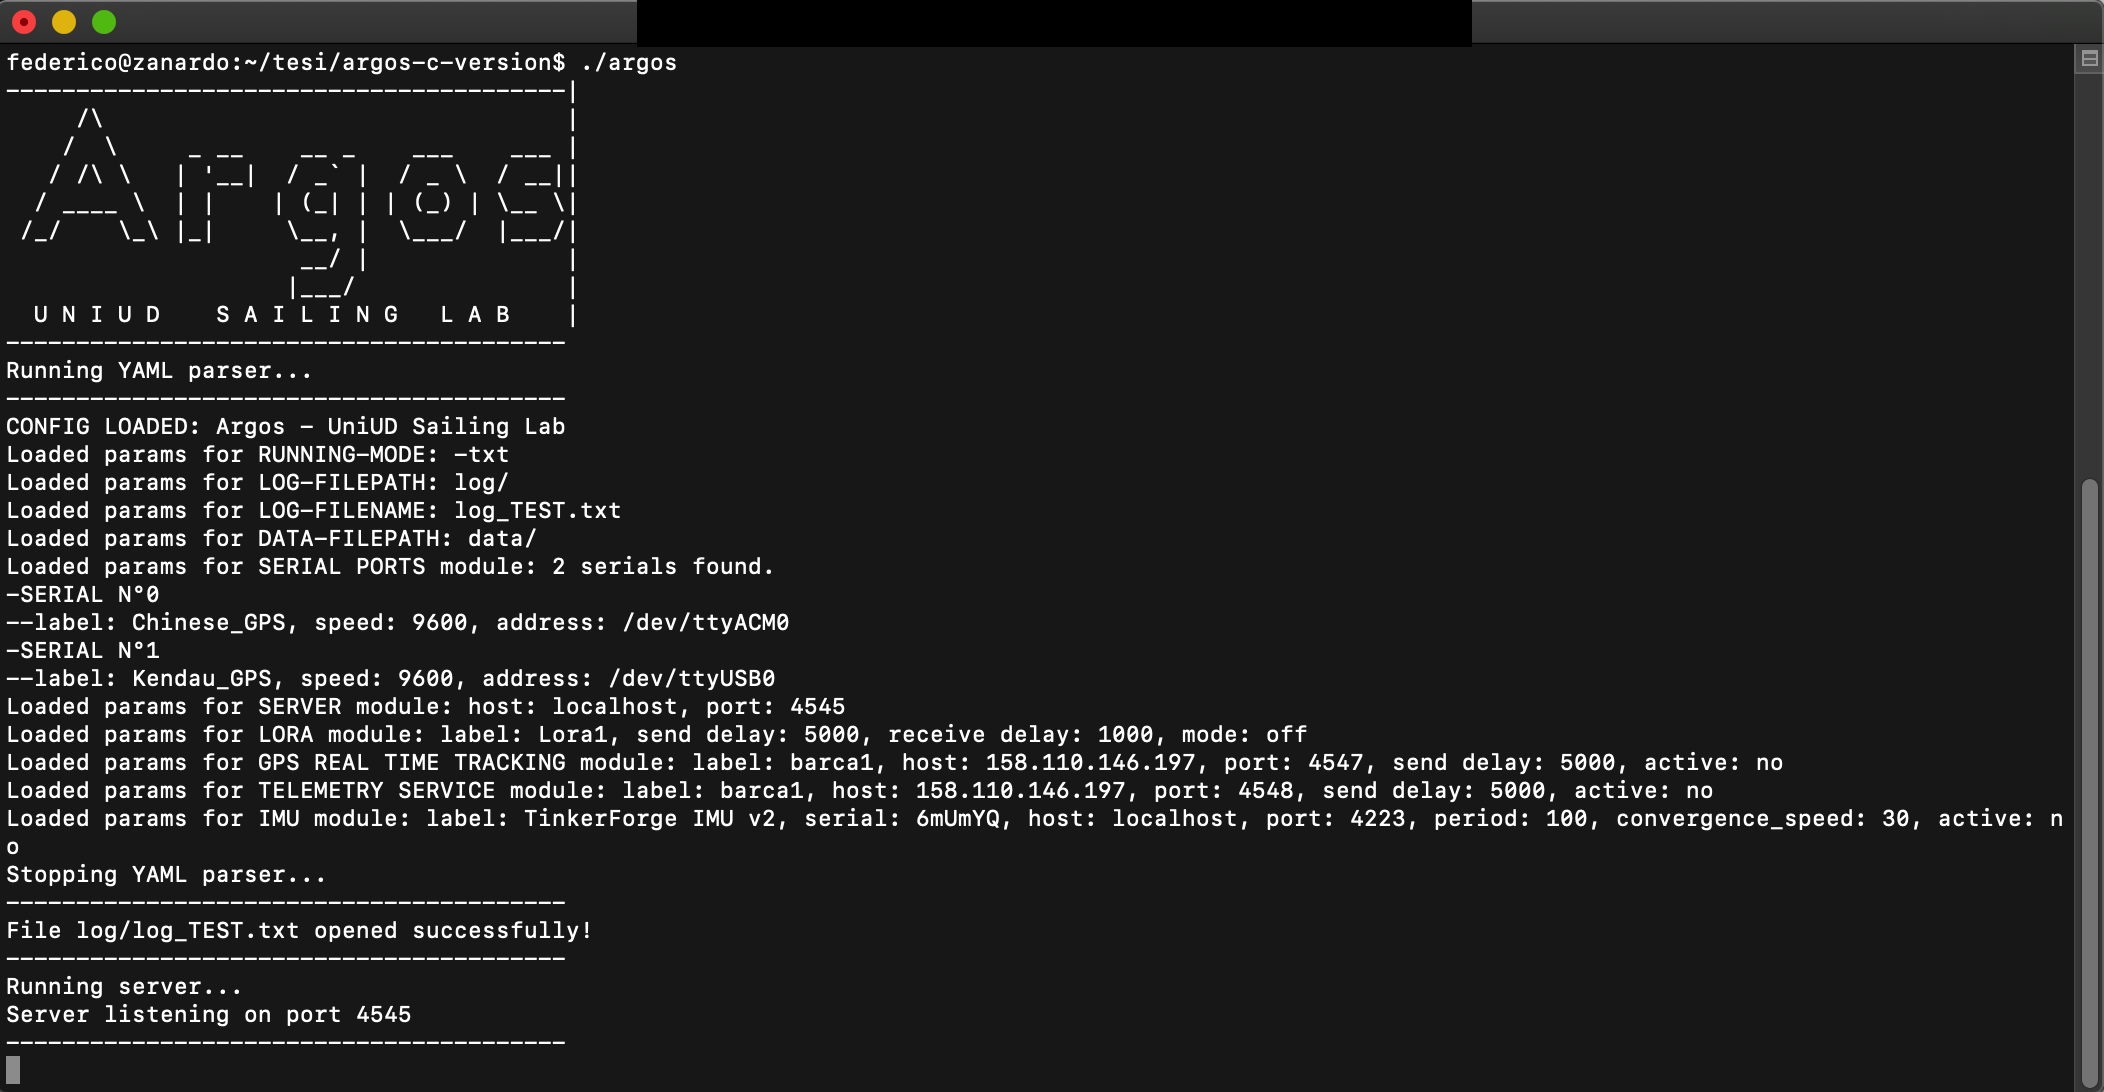
\includegraphics[scale=0.4]{argos}
		\caption[Argos]{La seconda versione del server \textit{Argos} in esecuzione.}
		\label{figura:argos}
	\end{center}
\end{figure}

\newpage

\subsubsection{Dati rilevati dai sensori ed elaborati dal server}
I dati che vengono rilevati dai sensori e poi inviati al server, vengono salvati su un file nel formato JSON. I sensori notificano periodicamente il server della disponibilità di nuovi dati: in questo modo l'utente avrà a disposizione sempre un set di dati aggiornati. Oltre ai dati forniti dai sensori, il server mette a disposizione degli ulteriori dati necessari per effettuare il \textit{debugging}. Tali dati per il debugging vengono forniti dalla socket insieme a tutti gli altri dati dei sensori, senza la necessità di dover effettuare delle particolari richieste.

Di seguito verrà fornita una descrizione di alcuni dei dati che vengono raccolti dai sensori e poi resi disponibili dal server:
\begin{enumerate}
	\item \textbf{A.W.S.} (Apparent Wind Speed): identifica la velocità del vento apparente o stimata;
	\item \textbf{A.W.A.} (Apparent Wind Angle): identifica l’angolo del vento apparente;
	\item \textbf{S.O.G.} (Speed Over Ground): indica la velocità effettiva della barca esente dagli effetti delle correnti marine;
	\item \textbf{C.O.G.} (Curse Over Ground): indica la direzione vera della barca, esente dagli effetti delle correnti marine. Rappresenta la rotta che sta percorrendo la barca;
	\item \textbf{M.H.} (Magnetic Heading): identifica il valore della direzione, segnalata dalla bussola di bordo;
	\item \textbf{S.O.W.} (Speed Over Water): rappresenta la velocità della barca sull’acqua;
	\item \textbf{T.W.S.} (True Wind Speed): indica la velocità attuale del vento;
	\item \textbf{T.W.A.} (True Wind Angle): rappresenta l'angolo percepito del vento;
	\item \textbf{I.H.} (Imu Heading): rappresenta la direzione data dalla IMU, l'angolo rispetto al Nord magnetico;
	\item \textbf{C.ANG.} (Calypso Ang): indica l'angolo con cui il vento arriva sullo strumento di misurazione \textit{Calypso}, ovvero, l’angolo misurato in base alla tacca segnata sullo strumento;
	\item \textbf{C.AMP.} (Calypso Amp): identifica la forza del vento, misurata in nodi, dallo strumento \textit{Calypso};
	\item \textbf{NWANG}: indica l'angolo del vento rispetto al Nord magnetico. È dato somma di \textit{IMU Heading} e \textit{Calypso Ang};
	\item \textbf{LATITUDE}:  latitudine;
	\item \textbf{LONGITUDE}: longitudine.
\end{enumerate}

Nell'applicazione finale, questi dati vengono distribuiti nelle varie schermate. Alcune schermate mostreranno un piccolo set di questi dati per focalizzarsi su determinati aspetti come la navigazione, il vento o le coordinate GPS. La dashboard invece offre un quadro generale della situazione, illustrando tutti i dati appena descritti.

I dati elencati non sono tutti quelli che vengono forniti dalla socket: i dati illustrati sono soltanto quelli che vengono utilizzati all'interno dell'applicazione.

\subsection{Neptune}
\subsubsection{Premessa}
Il lavoro riguardo alla realizzazione dell'applicazione Web è stata dapprima affrontata dallo studente \textit{Davide D'Osvaldo}. Un miglioramento di tale applicazione è stato effettuato prima da \textit{Edoardo Polce} e successivamente da \textit{Alessandro Martin}. Il mio lavoro ha preso in considerazione la versione dell'applicazione di quest'ultimo.

Lo sviluppo dell'applicazione per dispositivi Android è stato effettuato dallo studente \textit{Andrea Mazzocut}, di cui farò riferimento in questa sezione.

\subsubsection{Obiettivo dell'applicazione}
\textbf{Neptune} è un'applicazione lato client che permette di connettersi al server (tramite una socket alla porta \verb|4545|). Il client deve necessariamente essere connesso alla rete WiFi creata dal Raspberry. Ad intervalli regolari, l'applicazione interroga la socket per ottenere dei dati riguardanti i sensori installati sulla barca. Questi dati, in formato JSON, vengono mostrati in un'apposita interfaccia grafica. Nel corso di questo progetto, diversi studenti hanno partecipato alla realizzazione di differenti tipologie di applicazioni, per usufruire dei servizi offerti dal server Argos.

\subsubsection{Applicazione web}
\begin{figure}
	\begin{center}
		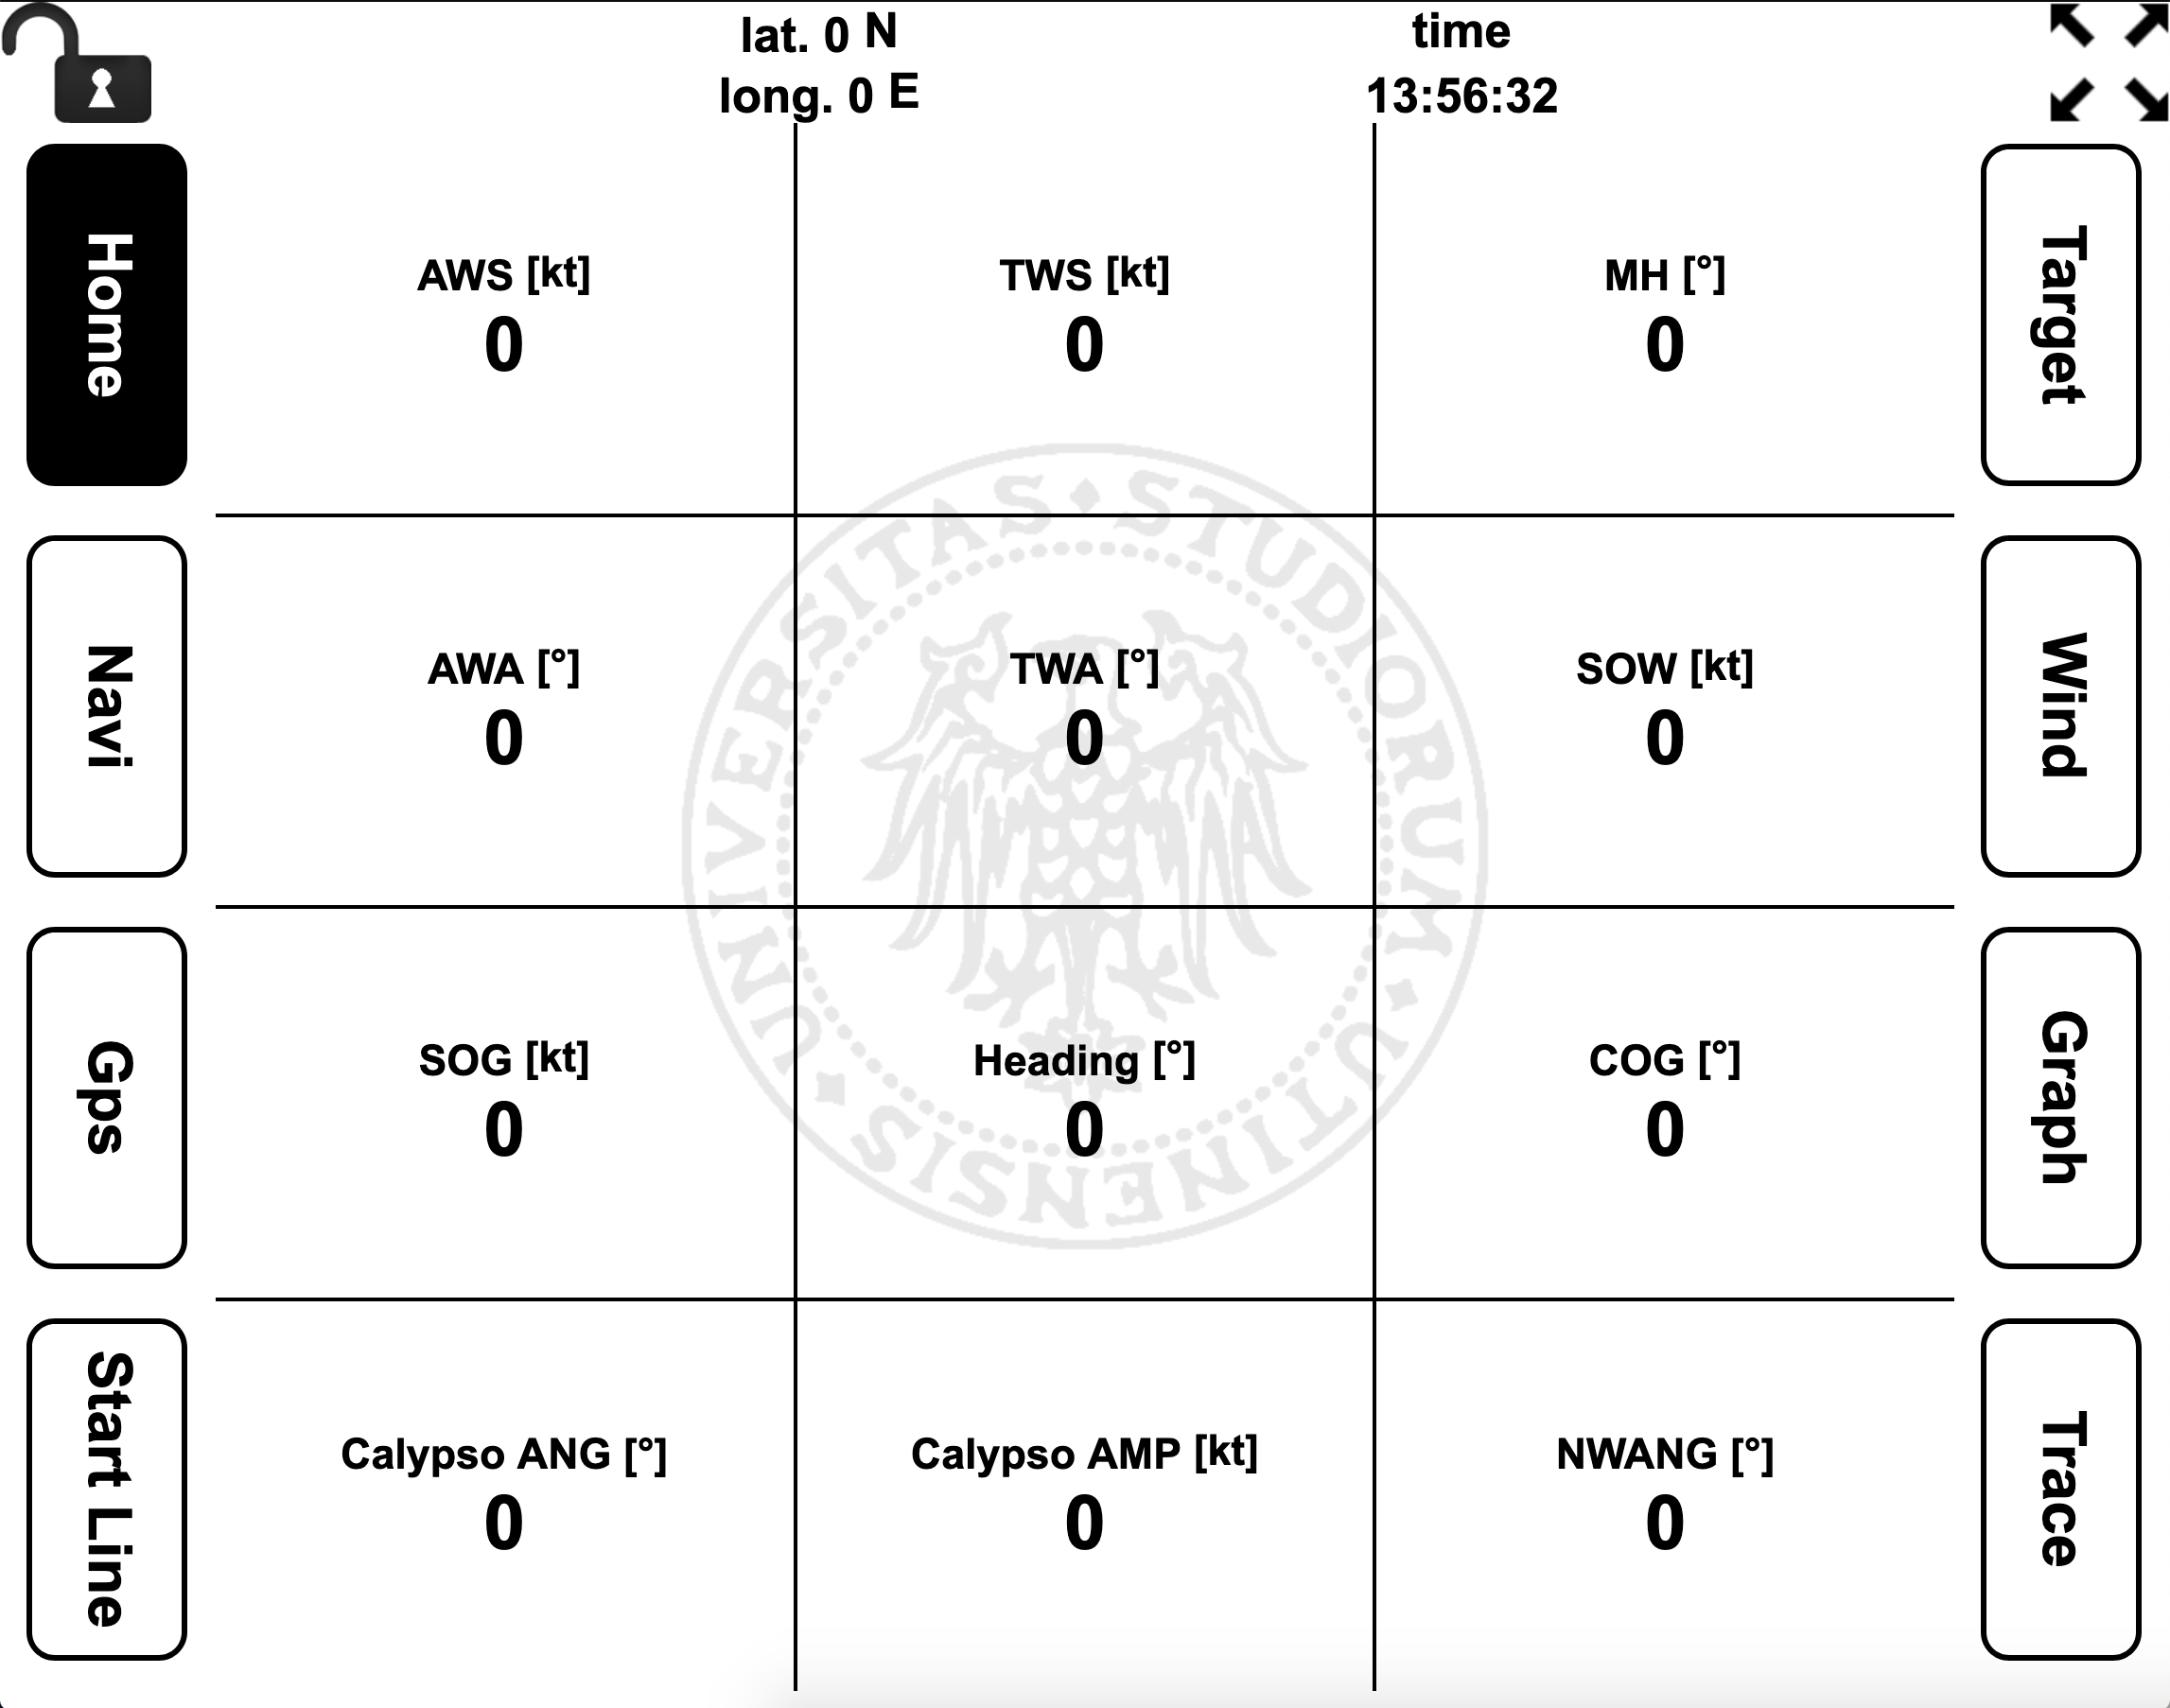
\includegraphics[scale=0.3]{neptune_web}
		\caption[Neptune - versione Web]{Schermata Home dell'applicazione Neptune nella versione Web.}
		\label{figura:neptune_web}
	\end{center}
\end{figure}

L'obiettivo di questa applicazione è la creazione di una sorta di \textit{computer di bordo} per essere utilizzato dall'equipaggio durante la competizione. L'accesso a Neptune è permesso a qualsiasi dispositivo che possa connettersi via wireless al Raspberry, in quanto l'applicazione è accessibile tramite il \textit{browser}.

L'applicazione è costituita da diverse schermate: in particolare, è possibile notare una schermata che presenta una serie di dati per avere un quadro generale di tutti i segnali provenienti dai sensori e delle altre schermate che permettono di monitorare dei dati specifici. Così facendo è possibile avere sia una panoramica generale dei dati rilevati dai sensori, sia un focus preciso su un piccolo set di dati.

Il software è stato sviluppato in HTML, CSS e JavaScript per la parte \textit{frontend}, mentre per la parte \textit{backend} è stato utilizzato PHP. Tuttavia questa versione dell'applicazione porta con sè diversi svantaggi, sopratutto a livello di uso pratico. Durante la regata, vengono utilizzati dei dispositivi mobili come smartphone e tablet, in modo da poterli maneggiare facilmente in ogni situazione e in ogni condizione. Di conseguenza, dispositivi di dimensioni maggiori rispetto a quelli citati sopra non vengono presi in considerazione. Per usufruire dell'applicazione Web è necessario quindi collegarsi via browser al sito web che ospita l'applicazione. L'esperienza utente per questa tipologia di software e per i dispositivi utilizzati non è ottimale, in quanto non vengono sfruttate appieno tutte le funzionalità native del dispositivo mobile.

\subsubsection{Applicazione Android}
Lo sviluppo di un'applicazione \textit{nativa} per dispositivi mobili con sistema operativo \textit{Android} è stata presa in considerazione per cercare di sopperire agli svantaggi della versione Web. L'applicazione nativa non ha l'intento di estendere o introdurre delle nuove funzionalità al servizio offerto, bensì l'intento è quello di rendere il servizio più facile da utilizzare e più reattivo in termini di prestazioni. Infatti, così facendo, è possibile sfruttare appieno le caratteristiche dei dispositivi mobili, permettendo un uso più naturale del servizio e riducendo anche i consumi delle risorse del dispositivo.
Sulla base di queste considerazioni, è possibile personalizzare meglio il servizio: ad esempio, in questa versione dell'applicazione, è stato possibile introdurre la funzionalità per cambiare l'indirizzo IP, quando lo si necessita. Nella versione Web questo poteva essere fatto soltanto dal programmatore che ha realizzato l'applicazione. La funzionalità appena descritta non ha un'importanza maggiore rispetto alle altre già esistenti, ma aiuta a migliorare il servizio nel caso in cui si renda necessario dover svolgere un'operazione di questo genere.

\begin{figure}[htp]
	\centering
	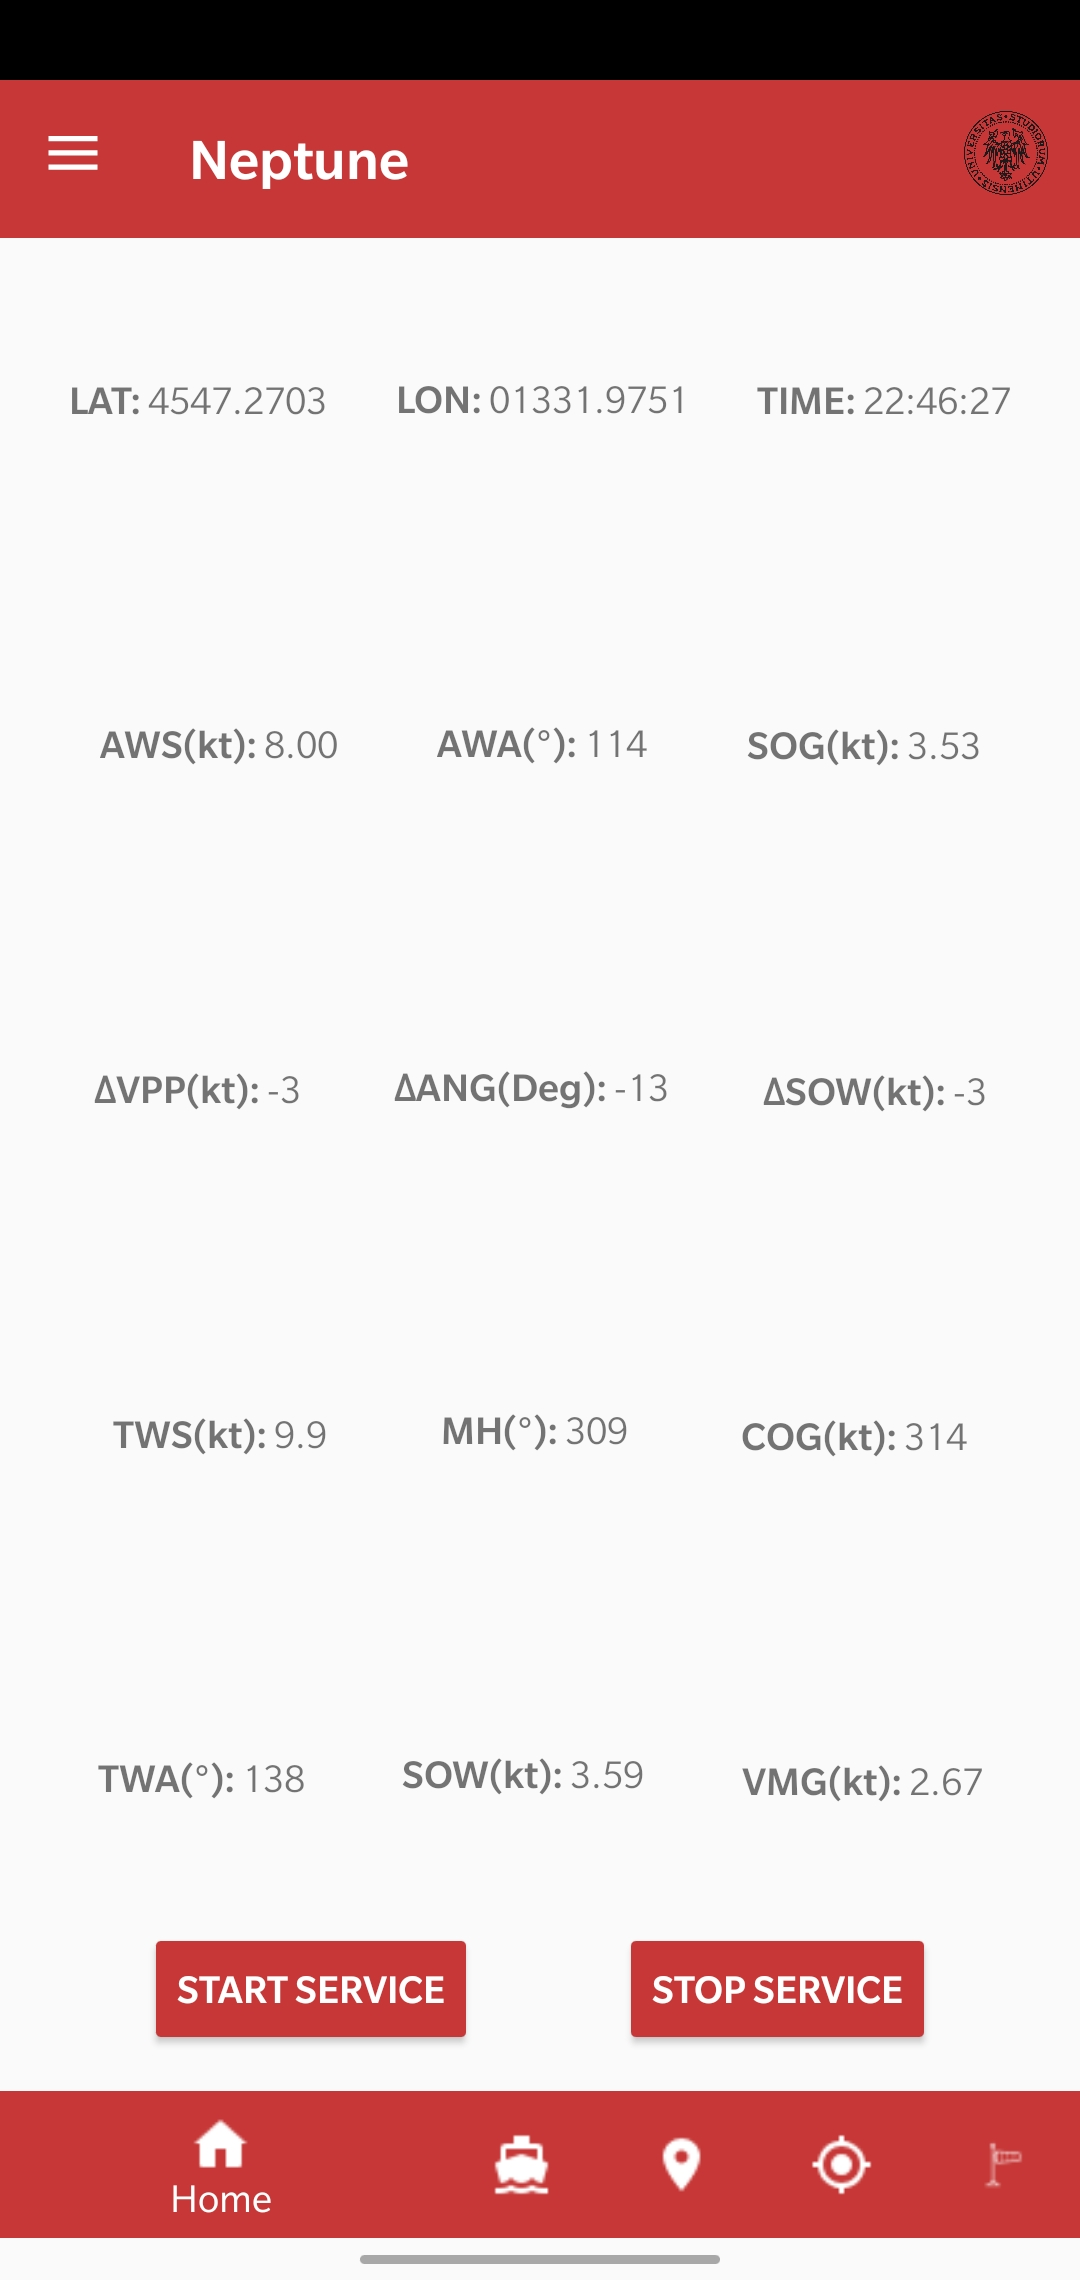
\includegraphics[scale=0.12]{neptune_home}\hfill
	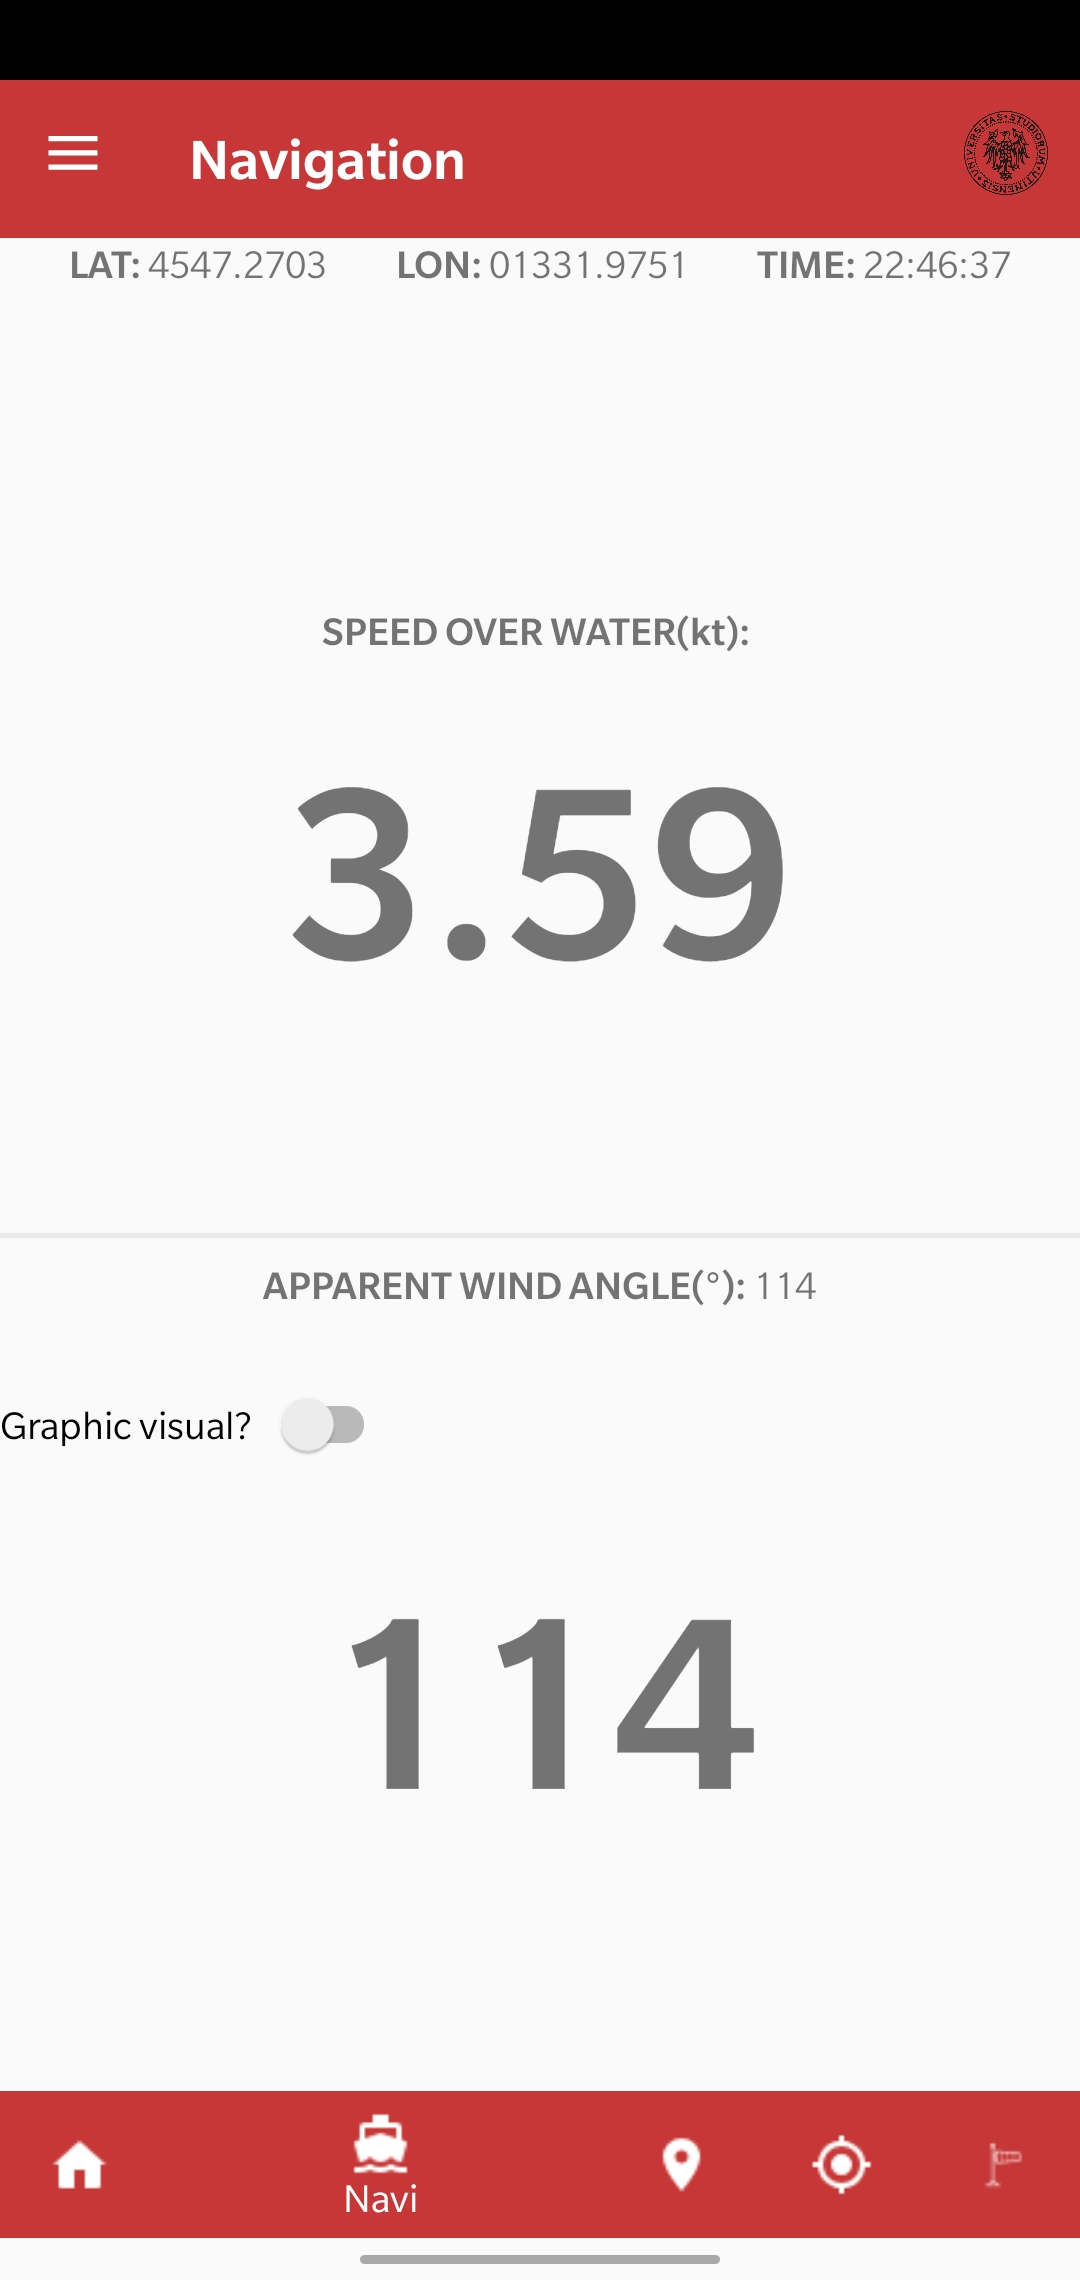
\includegraphics[scale=0.12]{neptune_navigation}\hfill
	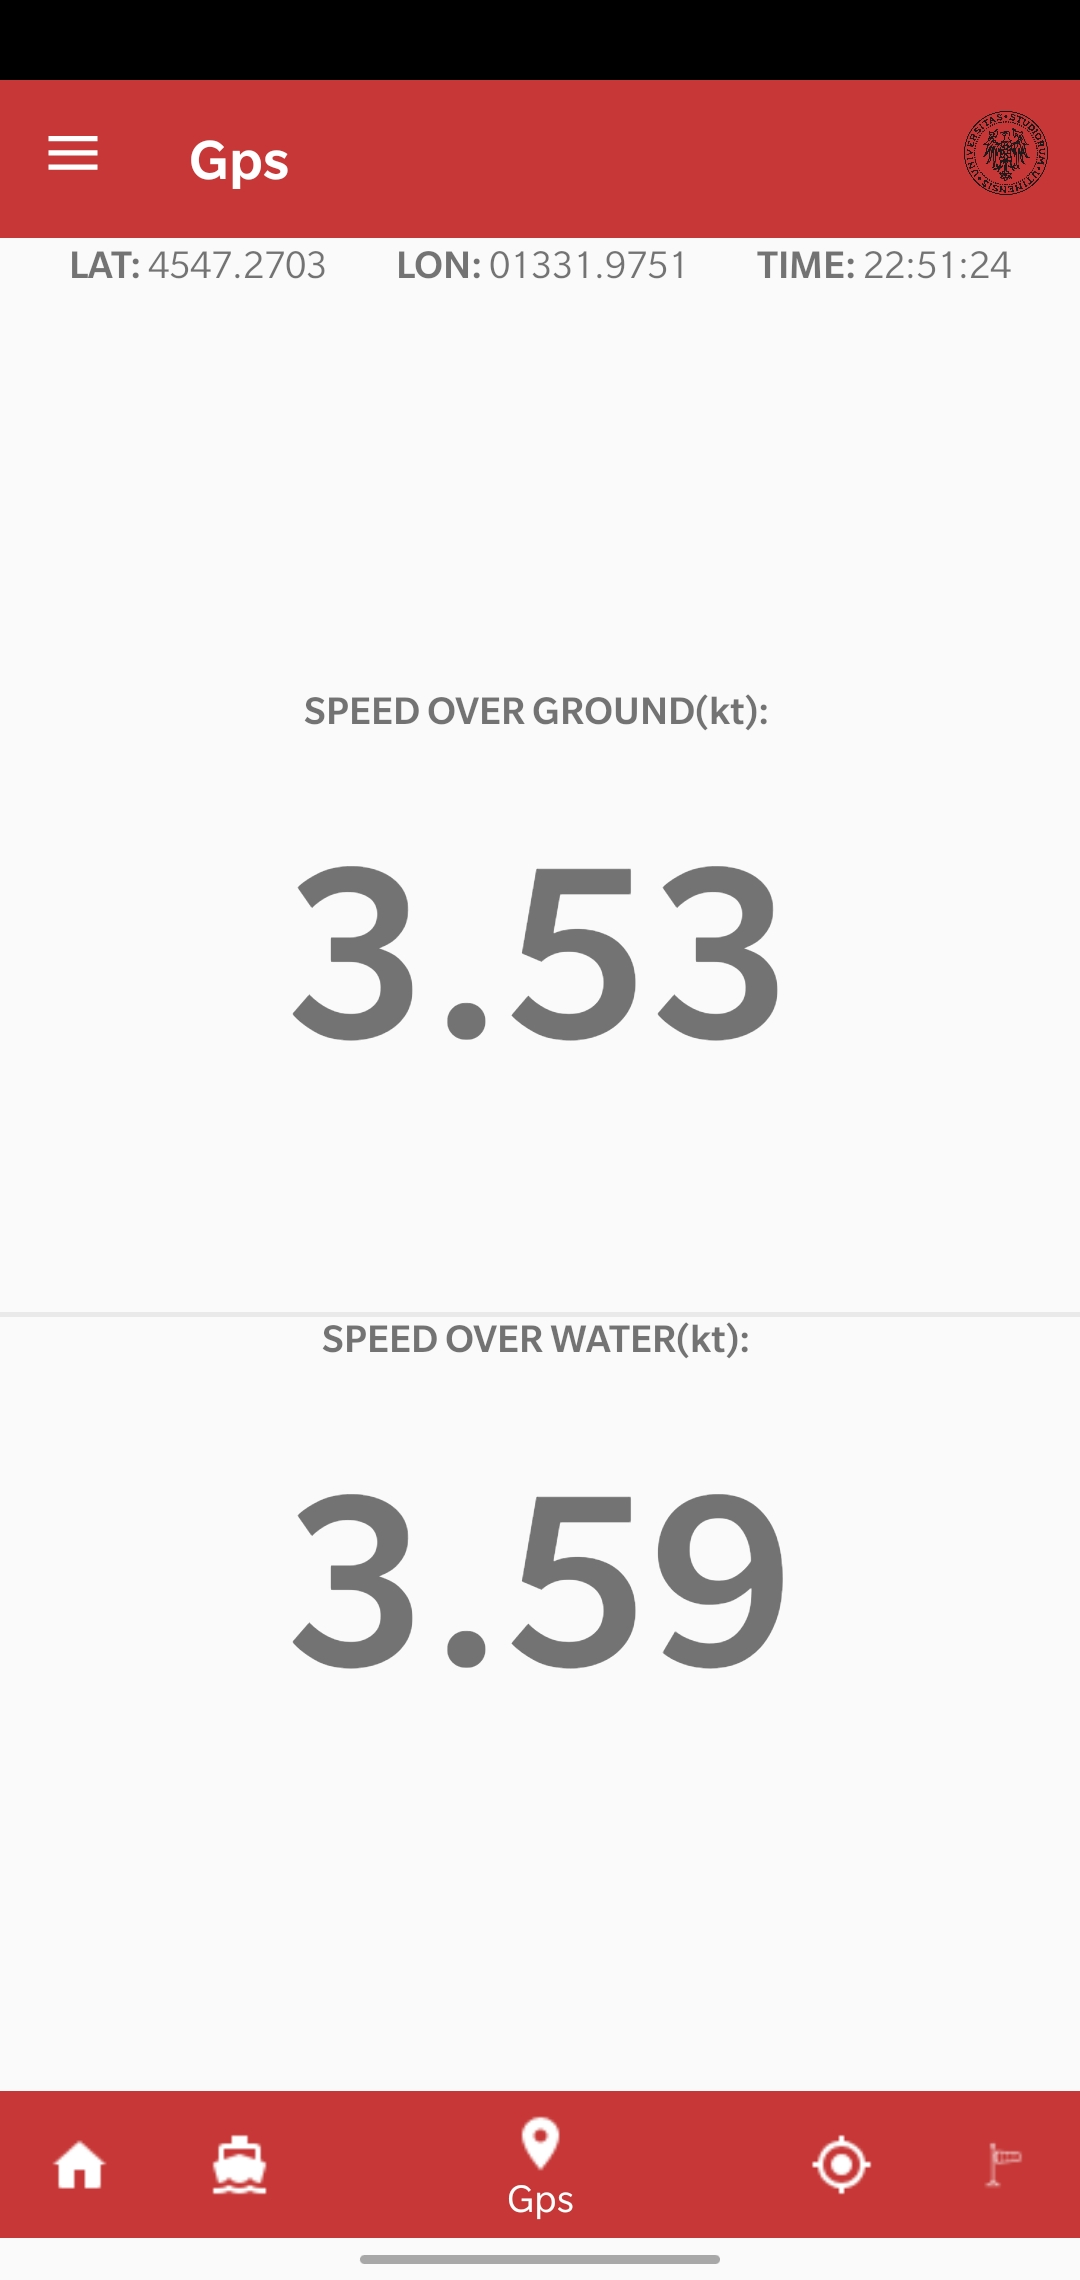
\includegraphics[scale=0.12]{neptune_gps}
	\caption[Neptune - versione Android]{Alcune schermate dell'applicazione Android: schermate Home, Navigation e GPS (in ordine da sinistra).}\label{xyz}
\end{figure}

